\section{Communication}
%%%%%%%%%%%% MID WAY AGENDA %%%%%%%%%%%%%%
\begin{frame}<beamer>
\frametitle{Communication overview}
  \begin{figure}
  \pause
  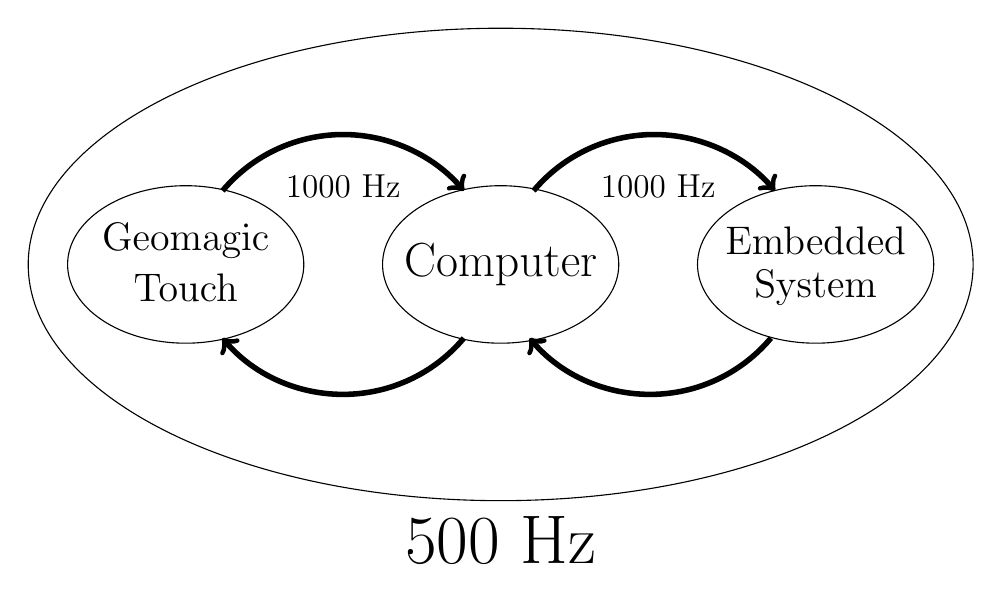
\begin{tikzpicture}

  \draw  (-3,0) ellipse (1.5 and 1)node (v1) {\LARGE Computer};
  \draw  (-7,0) ellipse (1.5 and 1)node{};
  \draw  (1,0) ellipse (1.5 and 1)node{};
  \node at (1,0.3) {\Large Embedded};
  \node at (1,-0.3) {\Large System};
  \node at (-7,0.3) {\Large Geomagic};
  \node at (-7,-0.3) {\Large Touch};

  \draw [->,line width=2pt](-6.5321,0.9356) arc (139.9997:40:2);
  \draw [<-,line width=2pt](-6.5321,-0.9356) arc (-139.9997:-40:2);
  \draw [<-,line width=2pt](-2.6321,-0.9356) arc (-139.9997:-40:2);
  \draw [->,line width=2pt](-2.5821,0.9356) arc (139.9997:40:2);


  \node at (-5,1) {\large 1000 Hz};
  \node at (-1,1) {\large 1000 Hz};
  \draw  (v1) ellipse (6 and 3);
  \node at (-3,-3.5) {\Huge 500 Hz};
  \end{tikzpicture}
  \end{figure}
\end{frame}

% the license
\begin{frame}<beamer>
\frametitle{Communication}


  \begin{itemize}
  \item Previous communication
    \begin{itemize}
      \item<1-> Maximum for the initial system: 100 Hz
      \item<1-> Utilized Transmission Control Protocol
      \end{itemize}
  \end{itemize}
  %\vspace(2em)
  \begin{itemize}
  \item<1-> Our approach:
      \begin{itemize}
        \item<1-> Reducing the size of exchanged data
        \item<1-> Changing the transport protocol
      \end{itemize}
  \end{itemize}
  \end{frame}






\begin{frame}<beamer>
\frametitle{Reducing the size of the packet}
\begin{figure}[h]
\centering
\begin{minipage}{.45\textwidth}
\resizebox{\textwidth}{!}{
  \begin{tikzpicture}
      \matrix(dict1)[matrix of nodes,ampersand replacement=\&, %below=of game,
          nodes={align=center,text width=2.5cm},
          row 1/.style={anchor=south},
          column 1/.style={nodes={text width = 1.5cm}}
      ]{
      0   \& \{"p4\_primary":\{\\
      };


      \matrix(dict2)[matrix of nodes,ampersand replacement=\&,%below=of game,
          nodes={align=center,text width=2.5cm},
          row 1/.style={anchor=south},
          column 1/.style={nodes={text width = 1.5cm}},
          column 3/.style={nodes={text width = 4cm}}
      ] at ($(dict1)+ (2.1,-1)$){
      15  \& "positions": \& array of 4 positions\\
      };

      \matrix(dict3)[matrix of nodes,ampersand replacement=\&,%below=of game,
          nodes={align=center,text width=2.5cm},
          row 1/.style={anchor=south},
          column 1/.style={nodes={text width = 1.5cm}},
          column 3/.style={nodes={text width = 4cm}}
      ] at ($(dict2)+ (0,-1)$){
      125 \& ,"velocities": \& array of 4 velocities\\
      };

      \matrix(dict4)[matrix of nodes,ampersand replacement=\&,%below=of game,
          nodes={align=center,text width=2.5cm},
          row 1/.style={anchor=south},
          column 1/.style={nodes={text width = 1.5cm}},
          column 3/.style={nodes={text width = 4cm}}
      ] at ($(dict3)+ (0,-1)$){
      236 \& ,"efforts": \& array of 4 efforts\\
      };

      \matrix(dict5)[matrix of nodes,ampersand replacement=\&,%below=of game,
          nodes={align=center,text width=2.5cm},
          row 1/.style={anchor=south},
          column 1/.style={nodes={text width = 1.5cm}}
      ] at ($(dict4)+ (-2.1,-1)$){
      344 \& \}\} \\
      };

  %Boxes
      \draw(dict1-1-2.north east)--(dict1-1-2.north west)--(dict1-1-2.south west)--(dict1-1-2.south east)--(dict1-1-2.north east);
      \draw(dict2-1-2.north east)--(dict2-1-2.north west)--(dict2-1-2.south west)--(dict2-1-2.south east)--(dict2-1-2.north east);
      \draw(dict3-1-2.north east)--(dict3-1-2.north west)--(dict3-1-2.south west)--(dict3-1-2.south east)--(dict3-1-2.north east);
      \draw(dict4-1-2.north east)--(dict4-1-2.north west)--(dict4-1-2.south west)--(dict4-1-2.south east)--(dict4-1-2.north east);
      \draw(dict5-1-2.north east)--(dict5-1-2.north west)--(dict5-1-2.south west)--(dict5-1-2.south east)--(dict5-1-2.north east);


      \draw(dict2-1-3.north east)--(dict2-1-3.north west)--(dict2-1-3.south west)--(dict2-1-3.south east)--(dict2-1-3.north east);
      \draw($(dict3-1-3.north east)+(0,-0.03)$)--($(dict3-1-3.north west)+(0,-0.03)$)--(dict3-1-3.south west)--(dict3-1-3.south east)--($(dict3-1-3.north east)+(0,-0.03)$);
      \draw($(dict4-1-3.north east)+(0,-0.03)$)--($(dict4-1-3.north west)+(0,-0.03)$)--(dict4-1-3.south west)--(dict4-1-3.south east)--($(dict4-1-3.north east)+(0,-0.03)$);

  %curly braces
    \draw [decorate,decoration={brace,amplitude=10pt, mirror},xshift=-4pt,yshift=0pt]
    ($(dict2.north west)+(0.5,0)$) -- ($(dict4.south west)+(0.5,0)$) node [black,midway,xshift=-0.9cm] {\footnotesize Data};

    \draw [decorate,decoration={brace,amplitude=5pt, mirror},xshift=-4pt,yshift=0pt]
    ($(dict1.north west)+(0.5,0)$) -- ($(dict1.south west)+(0.5,0)$) node [black,midway,xshift=-0.9cm] {\footnotesize Head};

    \draw [decorate,decoration={brace,amplitude=5pt, mirror},xshift=-4pt,yshift=0pt]
    ($(dict5.north west)+(0.5,0)$) -- ($(dict5.south west)+(0.5,0)$) node [black,midway,xshift=-0.9cm] {\footnotesize Tail};

  %numbers
    \node at ($(dict1-1-1.north east)+(0,0.2)$) {\footnotesize 0};
    \node at ($(dict1-1-2.north east)+(0,0.2)$) {\footnotesize 15};

    \node at ($(dict2-1-1.north east)+(0,0.2)$) {\footnotesize 0};
    \node at ($(dict2-1-2.north east)+(0,0.2)$) {\footnotesize 12};
    \node at ($(dict2-1-3.north east)+(0,0.2)$) {\footnotesize 110};

    \node at ($(dict3-1-1.north east)+(0,0.2)$) {\footnotesize 0};
    \node at ($(dict3-1-2.north east)+(0,0.2)$) {\footnotesize 14};
    \node at ($(dict3-1-3.north east)+(0,0.2)$) {\footnotesize 112};

    \node at ($(dict4-1-1.north east)+(0,0.2)$) {\footnotesize 0};
    \node at ($(dict4-1-2.north east)+(0,0.2)$) {\footnotesize 11};
    \node at ($(dict4-1-3.north east)+(0,0.2)$) {\footnotesize 111};

    \node at ($(dict5-1-1.north east)+(0,0.2)$) {\footnotesize 0};
    \node at ($(dict5-1-2.north east)+(0,0.2)$) {\footnotesize 2};

      \node at ($(0,0.3)+(dict1-1-1.north)$) {bytes};
      \node at ($(0,0.6)+(dict1-1-1.north)$) {Offset};

  \end{tikzpicture}
  }
  \caption{Packet built using JSON}
  \label{fig:old_packets}
\end{minipage}
\begin{minipage}{.45\textwidth}
\centering
\vspace{25pt}
\resizebox{\textwidth}{!}{
  \begin{tikzpicture}
      \matrix(dict)[matrix of nodes,ampersand replacement=\&, %below=of game,
          nodes={align=center,text width=1.5cm},
          row 1/.style={anchor=south}%,
          column 1/.style={nodes={text width = 0.5cm, align=right}}
      ]{
      0   \& position1 \& position2 \& position3 \& position4\\
      16  \& velocity1 \& velocity2 \& velocity3 \& velocity4\\
      32  \& effort1   \& effort2   \& effort3   \& effort4\\
      48  \\
      };
      %horizontal
      \draw(dict-1-2.north west)--(dict-1-5.north east);
      \draw(dict-1-2.south west)--(dict-1-5.south east);
      \draw(dict-2-2.south west)--(dict-2-5.south east);
      \draw(dict-3-2.south west)--(dict-3-5.south east);
    %vertical
      \draw(dict-1-1.north east)--(dict-4-1.south east);
      \draw(dict-1-2.north east)--(dict-3-2.south east);
      \draw(dict-1-3.north east)--(dict-3-3.south east);
      \draw(dict-1-4.north east)--(dict-3-4.south east);
      \draw(dict-1-5.north east)--(dict-3-5.south east);

      %small at bottom
      \draw(dict-4-1.south east)--($(0.5,0)+(dict-4-1.south east)$);
      \draw($(0.5,0)+(dict-4-1.south east)$)--($(0.5,0.49)+(dict-4-1.south east)$);

      %numbers on top
      \node at ($(0,0.3)+(dict-1-1.north east)$) {0};
      \node at ($(0,0.3)+(dict-1-2.north east)$) {4};
      \node at ($(0,0.3)+(dict-1-3.north east)$) {8};
      \node at ($(0,0.3)+(dict-1-4.north east)$) {12};
      \node at ($(0,0.3)+(dict-1-5.north east)$) {16};

      \node at ($(0,0.3)+(dict-1-1.north)$) {bytes};
      \node at ($(0,0.6)+(dict-1-1.north)$) {Offset};

      %The zoom on the last byte
      \node (zoom) at (1,-2) {XXXX 4 booleans};
      \draw(zoom.north east)--(zoom.north west);
      \draw(zoom.north east)--(zoom.south east);
      \draw(zoom.north west)--(zoom.south west);
      \draw(zoom.south east)--(zoom.south west);
      \draw($(zoom.north)+(-0.35,0)$)--($(zoom.south)+(-0.35,0)$);
      \draw(zoom.north east)--($(1,0)+(dict-4-1)$);
      \draw(zoom.north west)--($(1,0)+(dict-4-1)$);
      \node at ($(zoom.north east)+(0,0.3)$) {1};
      \node at ($(zoom.north west)+(0,0.3)$) {0};

  \end{tikzpicture}
  }
  \caption{Packet built using the binary representation}
  \label{fig:new_packets}
\end{minipage}
\end{figure}
\begin{center}
  Size reduced by 85\%
  \end{center}
\end{frame}


\begin{frame}<beamer>
\frametitle{Communication protocol}

Changed from TCP/IP to UDP\vspace{1em}
\begin{itemize}
	\item Pros
	\begin{itemize}
	\item Less overhead
  \item Real time protocol   
	\end{itemize}
  \item Cons
  \begin{itemize}
  \item Connection less 
  \item Less reliable  
    %\item Results: maximum of 638 Hz
\end{itemize}
\end{itemize}
\end{frame}







\begin{frame}<beamer>
\frametitle{UDP implementation ROS}

\begin{figure}
\scalebox{0.75}{
\tikzstyle{box} = [draw,rounded corners, minimum height=15mm, minimum width=20mm, align=center, text centered]
\begin{tikzpicture}
\node[box] (Check_Send) at ($(0,0)$) {Check if there is\\new data to send};
\node[box] (Send) at ($(4.5,0)+(Check_Send)$) {Send};
\node[box] (Receive) at ($(4.5,0)+(Send)$) {Timed receive};
\node[box] (Check_Receive) at ($(0,-3.5)+(Receive)$) {Check if a packet\\was received};
\node[box] (Handle) at ($(-4.5,0)+(Check_Receive)$) {Convert the bitcode\\and make data available\\to higher levels};
\node[box] (Sleep) at ($(0,-3.5)+(Check_Send)$) {Sleep};
\draw[->, ultra thick] (Check_Send) -- (Send);
\draw[->, ultra thick] (Send) -- (Receive);
\draw[->, ultra thick]
  (Receive.south) -- (Check_Receive.north);
\draw[->, ultra thick] (Check_Receive) -- (Handle);
\draw[->, ultra thick] (Handle) -- (Sleep);
\draw[->, ultra thick] (Check_Send.north) -- ($(0,1.5)+(Check_Send)$)  -- ($(0,1.5)+(Receive)$) -- (Receive.north);
\draw[->, ultra thick] (Check_Receive.south) -- ($(0,-1.5)+(Check_Receive)$)  -- ($(0,-1.5)+(Sleep)$) -- (Sleep.south);
\draw[->, ultra thick] (Sleep.north)  -- (Check_Send.south);
 \node at ($(-0.5,1.2)+(Check_Send)$) {No};
 \node at ($(2.4,0.4)+(Check_Send)$) {Yes};
\node at ($(0.5,-1.2)+(Check_Receive)$) {No};
\node at ($(-2,0.4)+(Check_Receive)$) {Yes};
\end{tikzpicture}





% \begin{tikzpicture}

% \node[box] (Initialization) at (0,0) {Initialization};
% \node[box] (Check_Send) at ($(0,-2.5)+(Initialization)$) {Check if there is\\new data to send};
% \node[box] (Send) at ($(0,-2.5)+(Check_Send)$) {Send};
% \node[box] (Receive) at ($(0,-2.5)+(Send)$) {Timed receive};
% \node[box] (Check_Receive) at ($(0,-2.5)+(Receive)$) {Check if a packet\\was received};
% \node[box] (Handle) at ($(0,-2.5)+(Check_Receive)$) {Convert the bitcode\\and make data available\\to higher levels};
% \node[box] (Sleep) at ($(0,-2.5)+(Handle)$) {Sleep};


% \draw[->, ultra thick] (Initialization) -- (Check_Send);
% \draw[->, ultra thick] (Check_Send) -- (Send);
% \draw[->, ultra thick] (Send) -- (Receive);
% \draw[->, ultra thick] (Receive) -- (Check_Receive);
% \draw[->, ultra thick] (Check_Receive) -- (Handle);
% \draw[->, ultra thick] (Handle) -- (Sleep);

% \draw[->, ultra thick] (Check_Send.east) -- ++(1,0) |- (Receive.east);
% \draw[->, ultra thick] (Check_Receive.east) -- ++(1,0) |- (Sleep.east);
% \draw[->, ultra thick] (Sleep.west) -| ++(-2,0) |- (Check_Send);



% \node at ($(2.1,0.2)+(Check_Send)$) {No};
% \node at ($(0.4,-1)+(Check_Send)$) {Yes};

% \node at ($(2.1,0.2)+(Check_Receive)$) {No};
% \node at ($(0.4,-1)+(Check_Receive)$) {Yes};

% \end{tikzpicture}
}
\end{figure}

\end{frame}




\begin{frame}<beamer>
\frametitle{UDP implementation ROS}

\begin{figure}
\scalebox{0.75}{
\begin{tikzpicture}

\node[box] (Initialization) at (0,0) {Initialization};
\node[box] (Check_Send) at ($(0,-2.5)+(Initialization)$) {Check if there is\\new data to send};
\node[box] (Send) at ($(0,-2.5)+(Check_Send)$) {Send};
\node[box] (Receive) at ($(0,-2.5)+(Send)$) {Timed receive};
\node[box] (Check_Receive) at ($(0,-2.5)+(Receive)$) {Check if a packet\\was received};
\node[box] (Reset) at ($(0,-2.5)+(Check_Receive)$) {Reset the counter};
\node[box] (Handle) at ($(0,-2.5)+(Reset)$) {Convert the bitcode\\and make data available\\to higher levels};

\node[box] (Sleep) at ($(0,-2.5)+(Handle)$) {Sleep};

\node[box] (Increment) at ($(4.5,0)+(Reset)$) {Increment the counter};
\node[box] (Timeout) at ($(4.5,0)+(Handle)$) {if counter > 10,\\throw error};


\draw[->, ultra thick] (Initialization) -- (Check_Send);
\draw[->, ultra thick] (Check_Send) -- (Send);
\draw[->, ultra thick] (Send) -- (Receive);
\draw[->, ultra thick] (Receive) -- (Check_Receive);
\draw[->, ultra thick] (Check_Receive) -- (Reset);
\draw[->, ultra thick] (Reset) -- (Handle);
\draw[->, ultra thick] (Handle) -- (Sleep);

\draw[->, ultra thick] (Check_Send.east) -- ++(0.75,0) |- (Receive.east);
\draw[->, ultra thick] (Check_Receive.east) -| (Increment.north);
\draw[->, ultra thick] (Increment) -- (Timeout);
\draw[->, ultra thick] (Timeout.south) |- (Sleep);

\draw[->, ultra thick] (Sleep.west) -| ++(-2,0) |- (Check_Send);



\node at ($(2.1,0.2)+(Check_Send)$) {No};
\node at ($(0.4,-1)+(Check_Send)$) {Yes};

\node at ($(2.1,0.2)+(Check_Receive)$) {No};
\node at ($(0.4,-1)+(Check_Receive)$) {Yes};

\end{tikzpicture}
}
\end{figure}


\end{frame}




\begin{frame}<beamer>
\frametitle{UDP implementation sbRIO}

\begin{itemize}
\item Receive incoming data 
\item Get data from the test setup 
\item Convert and send data to ROS
\end{itemize}

\end{frame}





\begin{frame}<beamer>
\frametitle{Communication measurements}
\begin{center}
  $\begin{tabular}{|c|c|c|c|c|}
    \hline
    \text{Frequency (Hz)} & \text{delay (ms)} & \text{Jitter ($\mu$s)} & \text{Packet loss (\%)}\\
    \hline
    99 & 10.1 & 4.66E-2 & 0 \\
    \hline
    474 & 2.1 & 5.51E-2 & 0.2 \\
    \hline
    638 & 1.6 & 1.16E-2 & 1.2 \\
    \hline
  \end{tabular}$
  \captionof{table}{Measurements of the performances for the new communication protocol}
  \label{tab:new_protocol}
\end{center}
\end{frame}


